% !TeX program = xelatex
\documentclass[a4paper,10pt]{article}

% ============================================================================
% សន្លឹកកិច្ចការសិស្ស ស-ខ្មៅ (Student Fill-In Worksheet — No-LCD Classroom)
% មេរៀនទី១៦ (១៦.៤.២)៖ កន្លះបន្ទាត់ពុះក្រៅនិងក្នុង និងសំយោគមេរៀនទី១៦ (ត្រូវគ្នា ១០០% នឹង LS_Plan_EXB.tex)
% ============================================================================
\usepackage[a4paper, left=0.95cm, right=0.95cm, top=0.75cm, bottom=0.90cm, footskip=0.48cm]{geometry}
\usepackage{amsmath}
\usepackage{unicode-math}
\usepackage{fontspec}
\usepackage{array, colortbl}
\usepackage[table]{xcolor}
\usepackage{enumitem}
\usepackage{pifont}
\usepackage{fancyhdr}
\usepackage{lastpage}
\usepackage{tikz}
\usepackage[most]{tcolorbox}
\usetikzlibrary{calc, arrows.meta, angles, quotes, decorations.markings, babel}

\makeatletter
\let\@expl@@@mark@update@singlecol@structures@@\relax
\makeatother

% ============================================================================
% ការកំណត់ពុម្ពអក្សរ (Cross-Platform Font Resolver)
% ============================================================================
\providecommand{\NGSFindFonts}{%
  \IfFileExists{C:/Windows/Fonts/cambria.ttc}{%
    \def\NGSSysPath{C:/Windows/Fonts/}%
    \def\NGSUserPath{C:/Users/KIT/AppData/Local/Microsoft/Windows/Fonts/}%
  }{%
    \IfFileExists{./fonts/KhmerOSsiemreap.ttf}{\def\NGSSysPath{./fonts/}\def\NGSUserPath{./fonts/}}{%
    \IfFileExists{../fonts/KhmerOSsiemreap.ttf}{\def\NGSSysPath{../fonts/}\def\NGSUserPath{../fonts/}}{%
    \IfFileExists{../../fonts/KhmerOSsiemreap.ttf}{\def\NGSSysPath{../../fonts/}\def\NGSUserPath{../../fonts/}}{%
    \IfFileExists{../../../fonts/KhmerOSsiemreap.ttf}{\def\NGSSysPath{../../../fonts/}\def\NGSUserPath{../../../fonts/}}{%
    \IfFileExists{../../../../fonts/KhmerOSsiemreap.ttf}{\def\NGSSysPath{../../../../fonts/}\def\NGSUserPath{../../../../fonts/}}{%
    \IfFileExists{../../../../../fonts/KhmerOSsiemreap.ttf}{\def\NGSSysPath{../../../../../fonts/}\def\NGSUserPath{../../../../../fonts/}}{%
    \IfFileExists{../../../../../../fonts/KhmerOSsiemreap.ttf}{\def\NGSSysPath{../../../../../../fonts/}\def\NGSUserPath{../../../../../../fonts/}}{%
      \def\NGSSysPath{../../../../../../../fonts/}\def\NGSUserPath{../../../../../../../fonts/}%
    }}}}}}}%
  }%
}
\NGSFindFonts

\setmathfont[Path={\NGSSysPath}, FontIndex=1, Scale=1.02]{cambria.ttc}
\defaultfontfeatures{Ligatures=TeX}

\setmainfont[
  Path={\NGSUserPath},
  Extension=.ttf,
  Script=Khmer,
  BoldFont={KhmerOSsiemreap},
  BoldFeatures={FakeBold=1.8},
  ItalicFont={KhmerOSsiemreap},
  ItalicFeatures={FakeSlant=0.25},
  BoldItalicFont={KhmerOSsiemreap},
  BoldItalicFeatures={FakeBold=1.8, FakeSlant=0.25}
]{KhmerOSsiemreap}

\newfontfamily\muol[Path={\NGSUserPath}, Extension=.ttf, Script=Khmer]{KhmerOSmuollight}
\newfontfamily\TimesEn[Path={\NGSSysPath}, Extension=.ttf, BoldFont={timesbd}, ItalicFont={timesi}, BoldItalicFont={timesbi}]{times}

\XeTeXlinebreaklocale "km"
\XeTeXlinebreakskip = 0pt plus 1pt minus 0.1pt

\definecolor{panelgray}{gray}{0.93}
\definecolor{headgray}{gray}{0.85}

\pagestyle{fancy}
\fancyhf{}
\renewcommand{\headrulewidth}{0pt}
\fancyfoot[L]{\fontsize{8pt}{10pt}\selectfont អនុវិទ្យាល័យព្រះក្រសាំង \en{---} គណិតវិទ្យា ថ្នាក់ទី៨ \en{|} មេរៀនទី១៦ (១៦.៤ កន្លះបន្ទាត់ពុះក្រៅនិងក្នុង និងសំយោគមេរៀនទី១៦)}
\fancyfoot[R]{\fontsize{8.2pt}{10pt}\selectfont ទំព័រ \en{\thepage\ / \pageref{LastPage}}}

\setlength{\parindent}{0pt}
\setlength{\parskip}{0pt}
\setlength{\tabcolsep}{4pt}

\newcommand{\en}[1]{{\TimesEn #1}}
\newcommand{\enbf}[1]{{\TimesEn\textbf{#1}}}
\newcommand{\unit}[1]{\,\text{\en{#1}}}
\newcommand{\cnum}[1]{\mbox{\fontsize{10pt}{12pt}\selectfont\ding{\numexpr181+#1\relax}}}
\newcommand{\chkbox}{\tikz[baseline=-0.15ex]\draw[black, line width=0.85pt] (0,0) rectangle (0.25cm,0.25cm);}
\newcommand{\blank}[1]{\makebox[#1]{\dotfill}}
\newcommand{\tri}[1]{\ensuremath{\triangle #1}}
\newcommand{\ang}[1]{\ensuremath{\angle #1}}
\newcommand{\cg}{\ensuremath{\cong}}

\newcommand{\rightbox}[4][0.18]{%
  \draw[black, line width=0.8pt]
    ($(#3)!#1!(#2)$) -- ($($(#3)!#1!(#2)$)+($(#3)!#1!(#4)$)-(#3)$) -- ($(#3)!#1!(#4)$);
}

\newcommand{\secbar}[2]{%
  \vspace{3pt}%
  \begin{tcolorbox}[
    enhanced, sharp corners, colback=headgray, colframe=black,
    boxrule=0.9pt, boxsep=1pt, top=2.5pt, bottom=2.5pt, left=6pt, right=6pt,
    after skip=3pt
  ]
    {\muol\fontsize{9.2pt}{13.5pt}\selectfont #1}\hfill{\fontsize{8.3pt}{11.5pt}\selectfont\textbf{#2}}
  \end{tcolorbox}%
}

\tikzset{
  tk1/.style={postaction={decorate},decoration={markings,mark=at position 0.50 with {\draw[black, line width=0.90pt](0,-0.095)--(0,0.095);}}},
  tk2/.style={postaction={decorate},decoration={markings,
    mark=at position 0.45 with {\draw[black, line width=0.90pt](0,-0.095)--(0,0.095);},
    mark=at position 0.55 with {\draw[black, line width=0.90pt](0,-0.095)--(0,0.095);}}}
}

\newcolumntype{L}[1]{>{\raggedright\arraybackslash}p{#1}}
\newcolumntype{C}[1]{>{\centering\arraybackslash}p{#1}}

\begin{document}
\fontsize{9.4pt}{13.8pt}\selectfont

% ============================================================================
% ទំព័រទី ១៖ ក្បាលសន្លឹកកិច្ចការ + E1 + E2 (ពិសោធផ្ចិត J & សម្រាយបំភ្លឺ) + E3 (ទ្រឹស្ដីបទ & តារាងសំយោគផ្ចិត ៥)
% ============================================================================
\begin{tcolorbox}[
  enhanced, sharp corners, colback=white, colframe=black,
  boxrule=1.1pt, boxsep=2pt, top=5pt, bottom=5pt, left=6pt, right=6pt, after skip=6pt
]
  \begin{center}
    {\muol\fontsize{10pt}{14.5pt}\selectfont សន្លឹកកិច្ចការសិស្ស \enbf{---} គណិតវិទ្យា ថ្នាក់ទី៨ \enbf{(}១៦\enbf{.}៤ កន្លះបន្ទាត់ពុះក្រៅនិងក្នុង និងសំយោគមេរៀនទី១៦\enbf{)}}\\[2.5pt]
    {\fontsize{8.8pt}{12pt}\selectfont
    ឈ្មោះសិស្ស / ដៃគូ៖ \blank{6.2cm} \hspace{0.2cm}
    ថ្នាក់៖ \blank{1.4cm} \hspace{0.2cm}
    ក្រុម៖ \blank{1.2cm} \hspace{0.2cm}
    កាលបរិច្ឆេទ៖ \blank{2.8cm}}
  \end{center}
\end{tcolorbox}

% --- E1 Engage ---
\begin{tcolorbox}[
  enhanced, sharp corners, colback=panelgray, colframe=black,
  boxrule=0.8pt, boxsep=2pt, top=5pt, bottom=5pt, left=6pt, right=6pt, after skip=6pt
]
  \textbf{បេសកកម្មទី១ (\en{E1 - Engage})៖ ប៉មភ្លើងសញ្ញាសុវត្ថិភាព $J$ នៅក្រៅផ្លូវបំបែកត្រីកោណ $\tri{ABC}$}\\
  ផ្លូវត្រង់ទាំងបីបង្កើតបានកោះត្រីកោណ $\tri{ABC}$ ។ វិស្វករចង់ដាក់ប៉មភ្លើងសញ្ញា $J$ នៅ \textbf{ខាងក្រៅជ្រុង $BC$} (ក្នុងចន្លោះមុំ $\ang{BAC}$) ឱ្យស្មើចម្ងាយពីផ្លូវត្រង់ទាំងបី ($BC$, បន្លាយ $ABx'$ និងបន្លាយ $ACy'$) ។ ចូរទស្សន៍ទាយជាដៃគូ៖\\
  $\blacktriangleright$ តើកន្លះបន្ទាត់ណាខ្លះជួបគ្នាត្រង់ $J$? \;\chkbox\ ពុះក្រៅទាំង ៣ \hspace{0.2cm} \chkbox\ ពុះក្រៅនៃ $\ang{B},\ang{C}$ និងពុះក្នុងនៃ $\ang{A}$ \hspace{0.2cm} \chkbox\ គ្មានចំណុច $J$ ទេ
\end{tcolorbox}

% --- E2 Explore Part A: Excenter Discovery Lab ---
\secbar{ផ្នែកទី១ \enbf{(}ក\enbf{)} ៖ ពិសោធន៍ផ្ចិត $J$ និងរង្វង់ចារឹកក្នុងមុំក្រៅត្រីកោណ \enbf{(Excenter Lab --- E2)}}{ការងារជាដៃគូ \en{6 min}}

\noindent
\begin{minipage}[c]{9.0cm}
  \centering
  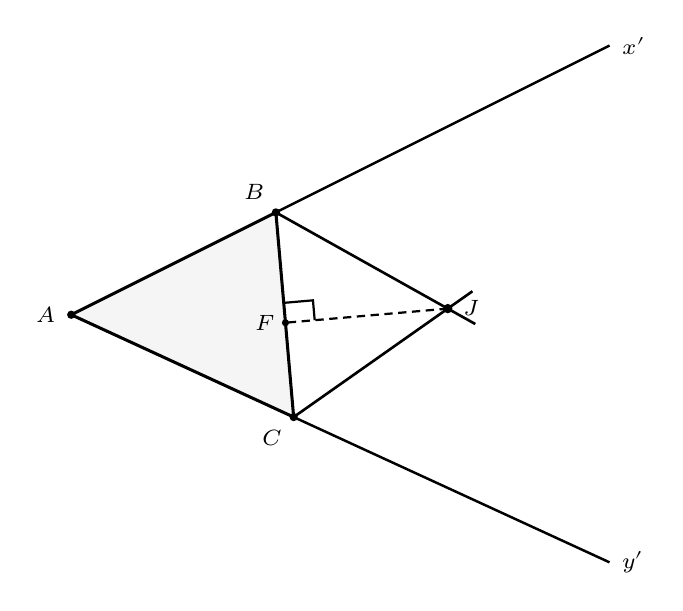
\begin{tikzpicture}[x=1.13cm, y=1.13cm, every node/.style={font=\footnotesize, text=black}]
    \coordinate (A) at (0,2.10);
    \coordinate (B) at (2.30,3.25);
    \coordinate (C) at (2.50,0.95);
    \coordinate (Bx) at (6.05,5.125);
    \coordinate (Cy) at (6.05,-0.683);

    \pgfmathsetmacro{\la}{veclen(0.20,-2.30)}
    \pgfmathsetmacro{\lb}{veclen(2.50,-1.15)}
    \pgfmathsetmacro{\lc}{veclen(2.30,1.15)}
    \pgfmathsetmacro{\den}{\lb+\lc-\la}
    \pgfmathsetmacro{\jx}{(-\la*0+\lb*2.30+\lc*2.50)/\den}
    \pgfmathsetmacro{\jy}{(-\la*2.10+\lb*3.25+\lc*0.95)/\den}
    \coordinate (J) at (\jx,\jy);
    \coordinate (F) at ($(B)!(J)!(C)$);

    \fill[gray!8] (A) -- (B) -- (C) -- cycle;
    \draw[black, line width=1.1pt] (A) -- (B) -- (C) -- cycle;
    \draw[black, line width=0.9pt] (B) -- (Bx) node[right=1pt] {$x'$};
    \draw[black, line width=0.9pt] (C) -- (Cy) node[right=1pt] {$y'$};
    \draw[black, line width=0.95pt] (B) -- ($(B)!1.16!(J)$);
    \draw[black, line width=0.95pt] (C) -- ($(C)!1.16!(J)$);
    \draw[black, line width=0.8pt, densely dashed] (J) -- (F);
    \rightbox[0.18]{J}{F}{B}

    \fill[black] (A) circle (1.5pt) node[left=2pt] {$A$};
    \fill[black] (B) circle (1.5pt) node[above left=1pt] {$B$};
    \fill[black] (C) circle (1.5pt) node[below left=1pt] {$C$};
    \fill[black] (J) circle (1.7pt) node[right=2pt] {$J$};
    \fill[black] (F) circle (1.3pt) node[left=1.5pt] {$F$};
  \end{tikzpicture}
\end{minipage}%
\hfill
\begin{minipage}[c]{9.6cm}
  \textbf{ជំហានពិសោធន៍ជាដៃគូលើរូបខាងឆ្វេង៖}\\[8pt]
  $1.$ ក្នុងរូបខាងឆ្វេង កន្លះបន្ទាត់ពុះក្រៅនៃ $\ang{B}$ និង $\ang{C}$ ជួបគ្នាត្រង់ $J$ ។ ចូរគូសភ្ជាប់កន្លះបន្ទាត់ $AJ$ រួចវាស់មុំដោយរ៉ាប់ព័រទ័រ៖\\
  \hspace*{0.35cm}$\ang{BAJ} = \blank{1.3cm}^\circ$ \hspace{0.2cm} និង \hspace{0.2cm} $\ang{CAJ} = \blank{1.3cm}^\circ$ ។\\
  \hspace*{0.35cm}$\Rightarrow$ តើ $AJ$ ជាកន្លះបន្ទាត់ពុះក្នុងនៃ $\ang{A}$ ដែរឬទេ? \chkbox\ មែន \;\chkbox\ មិនមែន\\[8pt]
  $2.$ យកអេគែរទម្លាក់កែង $JD \perp ABx'$ និង $JE \perp ACy'$ រួចវាស់៖\\
  \hspace*{0.35cm}$JF = \blank{1.2cm}\unit{cm}$, \; $JD = \blank{1.2cm}\unit{cm}$, \; $JE = \blank{1.2cm}\unit{cm}$ ។\\[8pt]
  $3.$ ឈានដែកឈានផ្ចិត $J$ កាំកែង $JF$ គូសរង្វង់! តើរង្វង់នេះប៉ះអង្កត់ $BC$ និងបន្ទាត់បន្លាយ $ABx', ACy'$ ដែរឬទេ? \chkbox\ ប៉ះទាំងបី \;\chkbox\ មិនប៉ះ
\end{minipage}

\vspace{16pt}
% --- E2 Explore Part B: Deductive Proof Fill-In ---
\secbar{ផ្នែកទី១ \enbf{(}ខ\enbf{)} ៖ សម្រាយបំភ្លឺតាមលក្ខណៈស្មើចម្ងាយ \enbf{---} ឧទាហរណ៍ ទំព័រ ២១១\enbf{--}២១២}{ការងារជាដៃគូ \en{5 min}}

$1.$ ដោយ $J$ នៅលើបន្ទាត់ពុះមុំក្រៅនៃ $\ang{B} \Rightarrow JD = \blank{1.0cm}$ ។ ដោយ $J$ នៅលើបន្ទាត់ពុះមុំក្រៅនៃ $\ang{C} \Rightarrow JF = \blank{1.0cm}$ ។\\[9.5pt]
$2.$ គេទាញបាន $JD = \blank{1.0cm}$ (ស្មើចម្ងាយពី $ABx'$ និង $ACy'$) $\Rightarrow J$ ឋិតលើ \textbf{\blank{2.8cm}} នៃមុំ $\ang{A}$ ក្នុង $\tri{ABC}$!\\[9.5pt]
$3.$ ដោយ $JD = JE = JF$ នោះ $D, E, F$ ស្ថិតលើរង្វង់ផ្ចិត $J$ ហៅថា \textbf{\blank{4.3cm}} (មាន \blank{0.8cm} រង្វង់ក្នុង ១ ត្រីកោណ) ។

\vspace{16pt}
% --- E3 Explain: Theorem & Master 5-Center Synthesis Table ---
\secbar{ផ្នែកទី២ ៖ ទ្រឹស្តីបទ និងតារាងសំយោគផ្ចិតពិសេសទាំង ៥ នៃមេរៀនទី១៦ \enbf{(E3 - Explain)}}{សង្ខេបរួមគ្នា \en{6 min}}

\begin{tcolorbox}[
  enhanced, sharp corners, colback=white, colframe=black,
  boxrule=0.9pt, boxsep=3pt, top=7pt, bottom=7pt, left=6pt, right=6pt
]
  $\bullet$ \textbf{ទ្រឹស្តីបទ (ទំ.២១២)៖} កន្លះបន្ទាត់ពុះក្រៅនៃមុំ \blank{1.2cm} របស់ត្រីកោណមួយ និងកន្លះបន្ទាត់ពុះក្នុងនៃមុំ \blank{1.3cm} ប្រសព្វគ្នាត្រង់ចំណុចតែមួយគត់ដែលស្មើចម្ងាយពីជ្រុងទាំងបី ហៅថា \textbf{\blank{4.6cm}} ($J$) ។\\[6.5pt]
  {\renewcommand{\arraystretch}{1.62}\footnotesize
  \begin{tabular}{|L{3.55cm}|C{1.05cm}|L{4.55cm}|L{7.95cm}|}
    \hline
    \cellcolor{headgray}\textbf{បន្ទាត់ពិសេសប្រសព្វគ្នា} & \cellcolor{headgray}\textbf{និមិត្ត.} & \cellcolor{headgray}\textbf{ឈ្មោះផ្ចិតពិសេស} & \cellcolor{headgray}\textbf{លក្ខណៈគន្លឹះ និងទីតាំងក្នុងត្រីកោណ} \\
    \hline
    $1.$ មេដ្យានទាំង ៣ (១៦.១) & $G$ & ទីប្រជុំទម្ងន់ & $AG = \blank{1.2cm}AA'$ (នៅខាងក្នុងជានិច្ច) \\
    \hline
    $2.$ មេដ្យាទ័រទាំង ៣ (១៦.២) & $O$ & ផ្ចិតរង្វង់ចារឹកក្រៅ & ស្មើចម្ងាយពី \blank{1.9cm} ($OA=OB=OC$) \\
    \hline
    $3.$ កម្ពស់ទាំង ៣ (១៦.៣) & $H$ & \blank{3.2cm} & កែងជ្រុងឈម (មុំទាល៖ នៅ \blank{1.6cm} ត្រីកោណ) \\
    \hline
    $4.$ ពុះមុំក្នុងទាំង ៣ (១៦.៤) & $I$ & ផ្ចិតរង្វង់ចារឹកក្នុង & ស្មើចម្ងាយពី \blank{1.9cm} ($IP=IQ=IR$; ក្នុងជានិច្ច) \\
    \hline
    $5.$ ពុះក្រៅ ២ + ពុះក្នុង ១ & $J$ & ផ្ចិតរង្វង់ចារឹកក្នុងមុំក្រៅ & $JD=JE=JF$ (នៅក្រៅជ្រុង; មាន ៣ ផ្ចិត $J, K, L$) \\
    \hline
  \end{tabular}}\\[6.5pt]
  $\bullet$ \textbf{ធនាគារហេតុផល៖}
  \cnum{1} ស្មើចម្ងាយបន្ទាត់ទ្រជ្រុង ($JD=JE=JF$) \;\textbar\;
  \cnum{2} ពុះក្នុង $\perp$ ពុះក្រៅ ($90^\circ$) \;\textbar\;
  \cnum{3} ទីប្រជុំទម្ងន់ $AG=\frac{2}{3}AA'$ \;\textbar\;
  \cnum{4} ផ្ចិតចារឹកក្រៅ $O$ \;\textbar\;
  \cnum{5} អរតូសង់ $H$
\end{tcolorbox}

\newpage

% ============================================================================
% ទំព័រទី ២៖ E4 (មុំត្រង់ I, J & លំហាត់ទី៨ ទំ.២១៣) + E5 (វិនិច្ឆ័យផ្ចិតទាំង ៥ & Exit Check) + កិច្ចការផ្ទះ
% ============================================================================

\secbar{ផ្នែកទី៣ ៖ ពង្រីកចំណេះដឹង និងសំយោគមេរៀនទី១៦ \enbf{(E4 - Elaborate)}}{អនុវត្ត \en{10 min}}

\noindent
\begin{minipage}[t]{9.2cm}\vspace{0pt}
  \begin{tcolorbox}[
    enhanced, sharp corners, colback=white, colframe=black, equal height group=rowE4,
    boxrule=0.85pt, boxsep=2.5pt, top=4pt, bottom=4pt, left=5pt, right=5pt
  ]
    \textbf{៣.ក ទំនាក់ទំនងរវាងផ្ចិត $I$ និងផ្ចិត $J$ ($\ang{A}=60^\circ$)៖}\\
    ក្នុង $\tri{ABC}$ មាន $\ang{A}=60^\circ$, $I$ ជាផ្ចិតរង្វង់ចារឹកក្នុង និង $J$ ជាផ្ចិតរង្វង់ចារឹកក្នុងមុំ $A$ ក្រៅ $\tri{ABC}$ ។
    \begin{center}
      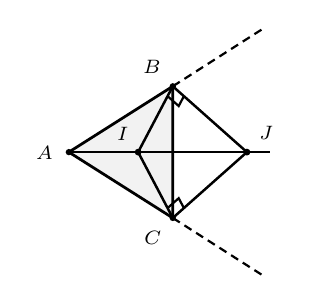
\begin{tikzpicture}[scale=0.88, every node/.style={font=\scriptsize, text=black}]
        \coordinate (A) at (-1.65,0);
        \coordinate (B) at (-0.15,0.95);
        \coordinate (C) at (-0.15,-0.95);
        \coordinate (I) at (-0.65,0);
        \coordinate (J) at (0.92,0);
        \fill[gray!10] (A) -- (B) -- (C) -- cycle;
        \draw[black, line width=1.0pt] (A) -- (B) -- (C) -- cycle;
        \draw[black, line width=0.8pt, densely dashed] (B) -- (1.15,1.78);
        \draw[black, line width=0.8pt, densely dashed] (C) -- (1.15,-1.78);
        \draw[black, line width=0.9pt] (A) -- (1.25,0);
        \draw[black, line width=0.9pt] (B) -- (I) -- (C) -- (J) -- (B);
        \rightbox[0.15]{I}{B}{J}
        \rightbox[0.15]{I}{C}{J}
        \fill[black] (A) circle (1.3pt) node[left=2pt] {$A$};
        \fill[black] (B) circle (1.3pt) node[above left=1pt] {$B$};
        \fill[black] (C) circle (1.3pt) node[below left=1pt] {$C$};
        \fill[black] (I) circle (1.4pt) node[above left=0.5pt] {$I$};
        \fill[black] (J) circle (1.4pt) node[above right=1pt] {$J$};
      \end{tikzpicture}
    \end{center}
    \vspace{-3pt}
    $1.$ ទាំង $I$ និង $J$ ស្ថិតលើកន្លះបន្ទាត់ពុះក្នុងនៃ $\ang{A}$ នាំឱ្យចំណុច $A, I, J$ \textbf{\blank{2.6cm}}!\\[3.5pt]
    $2.$ ដោយកន្លះបន្ទាត់ពុះក្នុង $BI$ កែងនឹងពុះក្រៅ $BJ$ គេបាន៖\\
    \hspace*{0.25cm}$\ang{IBJ} = \ang{ICJ} = \blank{1.1cm}^\circ$ (ហេតុផល \blank{0.65cm}) ។\\[3.5pt]
    $3.$ ដោយ $\ang{BIC} = 90^\circ + \frac{60^\circ}{2} = \blank{1.1cm}^\circ$ នោះក្នុងចតុកោណ $IBJC$ គេបាន៖ $\ang{BJC} = 180^\circ - \blank{1.1cm}^\circ = \blank{1.1cm}^\circ$!
  \end{tcolorbox}
\end{minipage}%
\hfill
\begin{minipage}[t]{9.6cm}\vspace{0pt}
  \begin{tcolorbox}[
    enhanced, sharp corners, colback=white, colframe=black, equal height group=rowE4,
    boxrule=0.85pt, boxsep=2.5pt, top=4pt, bottom=4pt, left=5pt, right=5pt
  ]
    \textbf{៣.ខ លំហាត់សំយោគទី៨ (ទំ.២១៣)៖ ចែកអង្កត់ទ្រូងជា ៣ ស្មើគ្នា}\\
    $ABCD$ ជាប្រលេឡូក្រាម, $I$ កណ្ដាល $AB$, $J$ កណ្ដាល $BC$, $P=AC\cap DI$, $Q=AC\cap DJ$ ។ បង្ហាញថា $AP=PQ=QC=\frac{AC}{3}$៖
    \begin{center}
      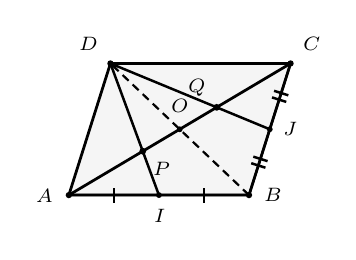
\begin{tikzpicture}[scale=0.88, every node/.style={font=\scriptsize, text=black}]
        \coordinate (A) at (-1.55,-0.95);
        \coordinate (B) at (1.05,-0.95);
        \coordinate (C) at (1.65,0.95);
        \coordinate (D) at (-0.95,0.95);
        \coordinate (I) at ($0.5*(A)+0.5*(B)$);
        \coordinate (J) at ($0.5*(B)+0.5*(C)$);
        \coordinate (O) at ($0.5*(A)+0.5*(C)$);
        \coordinate (P) at ($0.6667*(O)+0.3333*(A)$);
        \coordinate (Q) at ($0.6667*(O)+0.3333*(C)$);
        \fill[gray!8] (A) -- (B) -- (C) -- (D) -- cycle;
        \draw[black, line width=1.0pt] (A) -- (B) -- (C) -- (D) -- cycle;
        \draw[black, line width=1.0pt] (A) -- (C);
        \draw[black, line width=0.8pt, densely dashed] (B) -- (D);
        \draw[black, line width=0.9pt] (D) -- (I) (D) -- (J);
        \draw[black, line width=0.8pt, tk1] (A) -- (I);
        \draw[black, line width=0.8pt, tk1] (I) -- (B);
        \draw[black, line width=0.8pt, tk2] (B) -- (J);
        \draw[black, line width=0.8pt, tk2] (J) -- (C);
        \fill[black] (A) circle (1.3pt) node[left=2pt] {$A$};
        \fill[black] (B) circle (1.3pt) node[right=2pt] {$B$};
        \fill[black] (C) circle (1.3pt) node[above right=1pt] {$C$};
        \fill[black] (D) circle (1.3pt) node[above left=1pt] {$D$};
        \fill[black] (I) circle (1.2pt) node[below=1.5pt] {$I$};
        \fill[black] (J) circle (1.2pt) node[right=1.5pt] {$J$};
        \fill[black] (O) circle (1.2pt) node[above=2.5pt] {$O$};
        \fill[black] (P) circle (1.4pt) node[below right=0.5pt] {$P$};
        \fill[black] (Q) circle (1.4pt) node[above left=0.5pt] {$Q$};
      \end{tikzpicture}
    \end{center}
    \vspace{-3pt}
    -- គូស $BD$ កាត់ $AC$ ត្រង់ $O \Rightarrow AO = OC = \dfrac{1}{\blank{0.5cm}}AC$ ។\\[3.5pt]
    -- ក្នុង $\tri{ABD}$៖ មេដ្យាន $AO$ និង $DI$ ជួបត្រង់ $P$ ($\blank{2.2cm}$) $\Rightarrow AP = \frac{2}{3}AO = \frac{2}{3}\left(\frac{1}{2}AC\right) = \dfrac{AC}{\blank{0.5cm}}$ ។\\[3.5pt]
    -- ដូចគ្នាក្នុង $\tri{CBD}$៖ $QC = \dfrac{AC}{\blank{0.5cm}} \Rightarrow PQ = AC - AP - QC = \dfrac{AC}{\blank{0.5cm}}$!
  \end{tcolorbox}
\end{minipage}

\vspace{5pt}
% --- E5 Evaluate: 5-Center Diagnostic Matching + Exit Check ---
\secbar{ផ្នែកទី៤ ៖ វាយតម្លៃសំយោគមេរៀនទី១៦ \enbf{---} វិនិច្ឆ័យផ្ចិតទាំង ៥ និង \enbf{Exit Check (E5)}}{ធ្វើដោយឯករាជ្យ \en{10 min}}

\noindent
\begin{minipage}[t]{10.4cm}\vspace{0pt}
  \begin{tcolorbox}[
    enhanced, sharp corners, colback=white, colframe=black, equal height group=rowE5,
    boxrule=0.85pt, boxsep=2.5pt, top=4pt, bottom=4pt, left=5pt, right=5pt
  ]
    \textbf{៤.ក ល្បែងវិនិច្ឆ័យជ្រើសរើសផ្ចិតពិសេសទាំង ៥ ($G, O, H, I, J$)៖}\\
    ចូរបំពេញនិមិត្តសញ្ញាផ្ចិត ($G, O, H, I$ ឬ $J$) និងឈ្មោះបន្ទាត់ប្រសព្វឱ្យត្រូវតាមស្ថានភាព៖\\[4pt]
    {\renewcommand{\arraystretch}{1.48}\footnotesize
    \begin{tabular}{|L{5.65cm}|C{1.05cm}|L{2.15cm}|}
      \hline
      \cellcolor{headgray}\textbf{ស្ថានភាព / លក្ខណៈធរណីមាត្រ} & \cellcolor{headgray}\textbf{ផ្ចិត} & \cellcolor{headgray}\textbf{បន្ទាត់ប្រសព្វ} \\
      \hline
      $1.$ អណ្តូងទឹកស្មើចម្ងាយពីភូមិកំពូលទាំងបី $A, B, C$ & \blank{0.75cm} & \blank{1.85cm} \\
      \hline
      $2.$ ចំណុចទ្របន្ទះត្រីកោណឱ្យមានលំនឹងស្មើ & \blank{0.75cm} & \blank{1.85cm} \\
      \hline
      $3.$ ផ្ចិតអាងរង្វង់ខាងក្នុងប៉ះផ្លូវជ្រុងទាំងបី & \blank{0.75cm} & \blank{1.85cm} \\
      \hline
      $4.$ ប្រសព្វផ្លូវកែងគូសចេញពីកំពូលទៅជ្រុងឈម & \blank{0.75cm} & \blank{1.85cm} \\
      \hline
      $5.$ នៅក្រៅជ្រុង $BC$ តែស្មើចម្ងាយពីផ្លូវត្រង់ទាំងបី & \blank{0.75cm} & \blank{1.85cm} \\
      \hline
    \end{tabular}}
  \end{tcolorbox}
\end{minipage}%
\hfill
\begin{minipage}[t]{8.4cm}\vspace{0pt}
  \begin{tcolorbox}[
    enhanced, sharp corners, colback=white, colframe=black, equal height group=rowE5,
    boxrule=0.85pt, boxsep=2.5pt, top=4pt, bottom=4pt, left=5pt, right=5pt
  ]
    \textbf{៤.ខ សំណួរត្រួតពិនិត្យរហ័ស (\en{Exit Check})៖}\\
    គូសវង់ជុំវិញអក្សរនៃចម្លើយត្រឹមត្រូវតែមួយគត់៖\\[4.5pt]
    \textbf{សំណួរទី១ (បេសកកម្ម E1)៖} ផ្ចិតរង្វង់ចារឹកក្នុងមុំ $A$ ក្រៅ $\tri{ABC}$ ($J$) ជាប្រសព្វនៃ៖\\
    \hspace*{0.15cm}\textbf{ក.} មេដ្យាទ័រទាំង ៣ \hspace{0.35cm} \textbf{ខ.} ពុះមុំក្រៅទាំង ៣\\
    \hspace*{0.15cm}\textbf{គ.} ពុះក្រៅនៃ $\ang{B},\ang{C}$ និងពុះក្នុងនៃ $\ang{A}$\\[5.5pt]
    \textbf{សំណួរទី២៖} តើត្រីកោណមួយមានរង្វង់ចារឹកក្នុងមុំក្រៅចំនួនប៉ុន្មាន?\\
    \hspace*{0.15cm}\textbf{ក.} ១ រង្វង់ \hspace{0.55cm} \textbf{ខ.} ៣ រង្វង់ \hspace{0.55cm} \textbf{គ.} ៤ រង្វង់\\[5.5pt]
    \textbf{សំណួរទី៣៖} ក្នុងចំណោមផ្ចិតទាំង ៥ តើផ្ចិតណាខ្លះស្ថិតនៅខាងក្នុងត្រីកោណជានិច្ច (ទោះបីត្រីកោណមុំទាល)?\\
    \hspace*{0.15cm}\textbf{ក.} $G$ និង $I$ \hspace{0.45cm} \textbf{ខ.} $O$ និង $H$ \hspace{0.45cm} \textbf{គ.} $I$ និង $J$
  \end{tcolorbox}
\end{minipage}

\vspace{5pt}
% --- Step 5 Homework Box ---
\secbar{ផ្នែកទី៥ ៖ កិច្ចការផ្ទះបញ្ចប់មេរៀនទី១៦ និងការត្រៀមមេរៀនទី១៧ \enbf{(}ទំព័រ ២១៤\enbf{--}២១៧\enbf{)}}{ធ្វើនៅផ្ទះក្នុងសៀវភៅសរសេរ}

\begin{tcolorbox}[
  enhanced, sharp corners, colback=panelgray, colframe=black,
  boxrule=0.85pt, boxsep=3pt, top=4pt, bottom=4pt, left=6pt, right=6pt
]
  \begin{minipage}[c]{14.2cm}
    $1.$ \textbf{លំហាត់ទី១១ (ទំ.២១៤)៖} គេឱ្យ $ABCD$ ជាប្រលេឡូក្រាមមួយ គេកំណត់ $O$ ជាចំណុចប្រសព្វនៃអង្កត់ទ្រូងប្រលេឡូក្រាម, $H$ ជាអរតូសង់នៃ $\tri{ABC}$ និង $H'$ ជាអរតូសង់នៃ $\tri{ACD}$ ។ បង្ហាញថា $O$ ជាចំណុចកណ្ដាលនៃអង្កត់ $HH'$ \textit{(គន្លឹះ៖ បង្ហាញថា $AH\perp AD,\; CH'\perp AD \Rightarrow AH\parallel CH'$ និង $CH\parallel AH'$ រួចពិនិត្យអង្កត់ទ្រូងនៃប្រលេឡូក្រាម $AHCH'$)} ។\\[3pt]
    $2.$ \textbf{អានមេរៀនថ្មីជាមុន៖} \textbf{មេរៀនទី១៧ រូបធរណីមាត្រដែលមានវិមាត្របី} ចំណុច ១៧.១ ផ្ទៃក្រឡានៃព្រីស (ទំ.២១៥\,\en{--}\,២១៧) ។
  \end{minipage}%
  \hfill
  \begin{minipage}[c]{3.8cm}
    \centering
    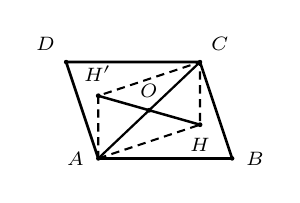
\begin{tikzpicture}[scale=0.68, every node/.style={font=\scriptsize, text=black}]
      \coordinate (A2) at (-0.95,-0.85);
      \coordinate (B2) at (1.55,-0.85);
      \coordinate (C2) at (0.95,0.95);
      \coordinate (D2) at (-1.55,0.95);
      \coordinate (O2) at (0,0.05);
      \coordinate (H) at (0.95,-0.22);
      \coordinate (Hp) at (-0.95,0.32);
      \fill[white] (A2) -- (B2) -- (C2) -- (D2) -- cycle;
      \draw[black, line width=0.95pt] (A2) -- (B2) -- (C2) -- (D2) -- cycle;
      \draw[black, line width=0.8pt] (A2) -- (C2);
      \draw[black, line width=0.9pt] (H) -- (Hp);
      \draw[black, line width=0.75pt, densely dashed] (A2) -- (H) -- (C2) -- (Hp) -- (A2);
      \fill[black] (A2) circle (1.2pt) node[left=1.5pt] {$A$};
      \fill[black] (B2) circle (1.2pt) node[right=1.5pt] {$B$};
      \fill[black] (C2) circle (1.2pt) node[above right=0.5pt] {$C$};
      \fill[black] (D2) circle (1.2pt) node[above left=0.5pt] {$D$};
      \fill[black] (O2) circle (1.3pt) node[above=1pt] {$O$};
      \fill[black] (H) circle (1.3pt) node[below=1.5pt] {$H$};
      \fill[black] (Hp) circle (1.3pt) node[above=1.5pt] {$H'$};
    \end{tikzpicture}
  \end{minipage}
\end{tcolorbox}

\end{document}
